\documentclass[a4paper,12pt]{book}
\bibliographystyle{junsrt}
\usepackage{ascmac}
\usepackage{empheq}
\usepackage{amsmath,amssymb}
\usepackage{bm}
\usepackage[dvipdfmx]{graphicx,color,hyperref}
\usepackage[top=30truemm,bottom=30truemm,left=30truemm,right=30truemm]{geometry}
\usepackage{braket}
\usepackage{here}
\usepackage{comment}
\usepackage{jtygm} % Warning
\usepackage[hang,small,bf]{caption}
\usepackage[subrefformat=parens]{subcaption}
\captionsetup{compatibility=false}
\title{Seismic Noise Under the Ground}
\author{Koseki Miyo}

% ハイパーリンクを付ける設定
\usepackage{pxjahyper}
\hypersetup{
  colorlinks=true,
  linkcolor=blue,
  %bookmarks=true, 
  bookmarksnumbered=true,
  pdfborder={0 0 0},
  bookmarkstype=toc
}


\begin{document}
\setcounter{tocdepth}{2}
\maketitle

\tableofcontents

\chapter{Seismic Noise Under the Ground}
\section{Introduction}
\subsection{Site on the Ground Surface}
\subsection{Site under the Ground}
\subsection{KAGRA Site}
\section{Theory of Seismic Waves}
\subsection{Seismic Waves}
\subsection{Depth Dependence}
\subsection{...}
\section{Seismic Noise}
\subsection{Problematic Seismic Noise}
\subsection{The Microseisms}

\subsection{The Earth Quakes}
I have to explain how earth quake shake the KAGRA site and how serious for interferometer.
\begin{itemize}
\item 
\item Mechanism and frequency of earthquake?
\end{itemize}

\subsection{The Earth Tide}

\begin{itemize}
  \item To explain accuracy of GIF in low frewuency comparign with seismometers, This subsection describe about the measurement of the Earth Tide using GIF, which is consistent with the GOTIC model.
\end{itemize}

\subsection{...}
\section{Seismic Noise Reduction in the Arm Cavity}
\subsection{Introduction}
The seismic noise shakes both the common and the differential motion of the arm cavity. The common motion moves the center of mass of that, and the differential motion moves the arm length. These motions are the same each other, when two mirrors in the cavity moves with no correlation. However, If there is the coherence, the differential motion is less than common motion. 

This coherence depends on both the arm length and the wave length of seismic motion which propagates along the arm. If the arm length is much smaller than the wave length, two mirrors in the cavity moves together. It means that the common motion is greater than differential motion. On the other hands, even though the arm length are the same in the gravitational-wave telescopes, the wave length are differed by the location because of different phase velocity on the ground. Especially for KAGRA, the velocity is much higher than other sites on surface of the ground due to hard rock of the gneiss. A ratio of the amplitudes of the differential motion over common motion on the ground is defined as Common and Differential Motion Ratio (CDMR). It is usefull value to know how the groung reduct the differential motion or how increase the common motion in the arm cavity. This redcution effects due to the propaty of the ground could relax to control the arm cavity.

In fact, we need to consider about the common motion because the arm length fluctuation is caused by not only the differential motion of the ground but also the coupling from the common motion to the length. This coupling ratio is kwnon as the Common Mode Rejection Ratio (CMRR). This is defined as the ratio of the powers of the differential-mode response over the common-mode response in a system. For example, in the case of ideal arm cavity, CMRR is infinity because the common response from the ground to optics is 0. However, in the actual case, the commom response is not 0 because there are some differencies in the responses of two mirrors. 

In this section, CDMR is discussed in detail, while CMRR of the arm cavity is in \ref{}.


\subsection{Differential Motion Reduction}
Motions of two mirrors in the arm cavity can be represented as the differential and the common motion. These motions are defined and calculated with the coherence between these two mirrors. 

In folowing disscusion, the mirrors are fixed on the ground and these of CMRR is high enough to ignore the coupling from common motion of ground to differential motion of the mirrors.

\subsubsection{Differential Motion and Common Motion}
\begin{figure}[H]
  \begin{center}
    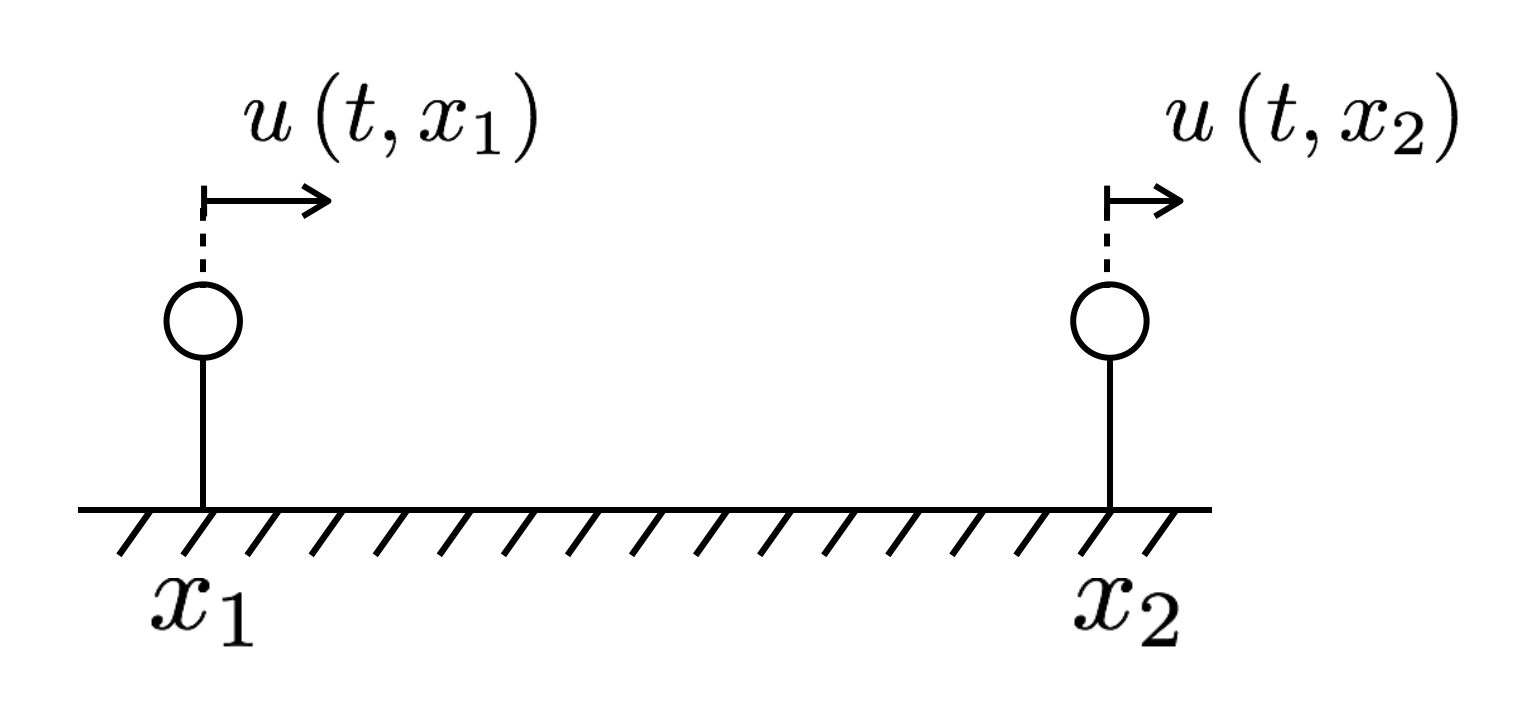
\includegraphics[width=8.0cm]{./img_cdmr_arm.png}
  \end{center}
  \caption{Displacements of two points,$x_1,\,x_2$. Displacements of each location are represented as $u(x_1,t),\, u(x_2,t)$, in the case displacement field is given with $u(x,t)$, where $x$ is location of the point and $t$ is a time.
  }\label{img:img_diffcomm}  
\end{figure}

Displacement of both differential motion and common motion of two points shown in Figure\ref{img:img_diffcomm} is defined as
\begin{eqnarray}\label{eq:eq22}
  u_{\mathrm{diff}} \equiv \frac{u_{1}-u_{2}}{\sqrt{2}}, \,
  u_{\mathrm{comm}}  \equiv \frac{u_{1}+u_{2}}{\sqrt{2}}
\end{eqnarray}
, where $u_{1}(x,t)$ and $u_2(x,t)$ are the displacement in each points.



\subsubsection{Common and Differential Motion Ratio (CDMR)}
Common and Differential Motion Ratio (CDMR) is defined as the powers of common motion over the differential motion as bellow,
\begin{equation}
  \mathrm{CDMR} \equiv \sqrt{\frac{\mathrm{Common\,Motion}}{\mathrm{Differential\,Motion}}} = \sqrt{\frac{P_{\mathrm{comm}}(\omega)}{P_{\mathrm{diff}}(\omega)}} \label{eq:eq23}
\end{equation}
,where $P_{\mathrm{comm}},P_{\mathrm{diff}}$ is the power spectrum densities (PSDs) of them. These are estimated by the autocorrelation function of these with the Wiener-Khinchin theorem.

Autocorrelation function $C_{\mathrm{diff}}$ is given by
\begin{eqnarray}
  C_{\mathrm{diff}}(\tau) &=& \frac{1}{2}
  \biggl\langle
  \biggl[ x_{1}(t)-x_{2}(t) \biggr] \biggl[ x_{1}(t+\tau)-x_{2}(t+\tau) \biggr]
  \biggr\rangle \\
  &=& \frac{1}{2}\biggl[ C_{11}(\tau) - C_{12}(\tau) - C_{21}(\tau) + C_{22}(\tau) \biggr], 
\end{eqnarray}
,where $C_{ij}$ are the autocorrelation functions of each location and defined as $ C_{ij} \equiv \langle x_{i}(t)x_{j}(t+\tau)\rangle,\, (i=1,2,\,j=1,2)$. Therefore, the power spectrum density of differential motion $P_{\mathrm{diff}}(\omega)$ can be computed as
\begin{eqnarray}
  P_{\mathrm{diff}}(\omega) &=& \frac{1}{2}\biggl[ P_{1}(\omega) + P_{2}(\omega) - P_{12}(\omega) - P_{12}^*(\omega) \biggr]\\
  &=& \frac{1}{2} \biggl[ P_{1}+P_{2} - \mathrm{Re}\left[\mathrm{coh} \right]\times2\sqrt{P_{1}P_{2}} \biggr] \label{eq:eq31}
\end{eqnarray}
where $P_{1}(\omega),P_{2}(\omega)$ are the power spectrum densities of each locations, and $P_{12}(\omega)$ are the cross spectrum between two location. $\mathrm{coh}$ is the complex coherence between them defined below.
\begin{eqnarray}
  \mathrm{coh} \equiv \frac{P_{12}}{\sqrt{P_{1}P_{2}}}
\end{eqnarray}

Assuming that $P_{1}=P_{2} \equiv P$, one can compute the CDMR using Eq.(\ref{eq:eq23}) as
\begin{eqnarray}
 \mathrm{CDMR} = \sqrt{\frac{1 + \mathrm{Re} \left[\mathrm{coh} \right] }{1 - \mathrm{Re} \left[\mathrm{coh} \right]}}. \label{eq:eq33}
\end{eqnarray}
Eq.(\ref{eq:eq33}) indicate that CDMR can be expressed by only the coherence between of two locations.

(aaaaa)

Incidentally, If the coherence is known and the PSDs of two location are same, one can estimate the PSDs of differential motion using that of one location according to Eq.(\ref{eq:eq31}) as
\begin{eqnarray}
  P_\mathrm{diff} = P \sqrt{1 - \mathrm{Re[coh]}}. \label{eq:eq34}
\end{eqnarray}
This expression is usefull to estimate a length fluctuation of the arm cavity even single point measurement because the coherence can be calculate using some models which is discussed following subsection.

\subsubsection{Single Plane Wave Model}
The CDMR when single plane wave propagates along the arm cavity is discussed. This model can be applied in the case the source of seismic motion is only one such as an earth quake. Assuming that the plane wave propagates with the azimuth angle $\theta$ along the direction of arm cavity, the wave length $\lambda$ is $\lambda/\mathrm{cos}\theta$. In this situation, the coherence from $x_1$ to $x_2$ is denoted as
\begin{equation}
  \mathrm{coh}=e^{i\frac{L\mathrm{cos}\theta\omega}{c}}
\end{equation}
Therefore, one can compute the CDMR as
\begin{equation}  \label{eq:eq18}
  \mathrm{CDMR} = \sqrt{\frac{1+\mathrm{cos}(\frac{L\omega}{c}\mathrm{cos}\theta)}{1-\mathrm{cos}(\frac{L\omega}{c}\mathrm{cos}\theta)}}.
\end{equation}


\subsubsection{Uniform Plane Wave Model}
The CDMR when the plane waves are distributed uniformly around the azimuth is discussed. This model can be applied in the case microseisms excite the ground. The coherence is equal to the integral over all direction.
\begin{eqnarray} \label{eq:eq19}
  \mathrm{coh} &=& \frac{1}{2\pi} \int_{-\pi}^{\pi} e^{i\frac{\omega}{c} L\cos \theta} d \theta
\end{eqnarray}
where the coherence is normized azimuth angle. Therefore, the CDMR is given as
\begin{equation}  \label{eq:eq20}
  \mathrm{CDMR} = \sqrt{\frac{1+J_0(\frac{L\omega}{c})}{1-J_0(\frac{L\omega}{c})}} .
\end{equation}


\subsubsection{Reduction Effect in the X-arm}

\begin{figure}[H]
  \begin{center}
    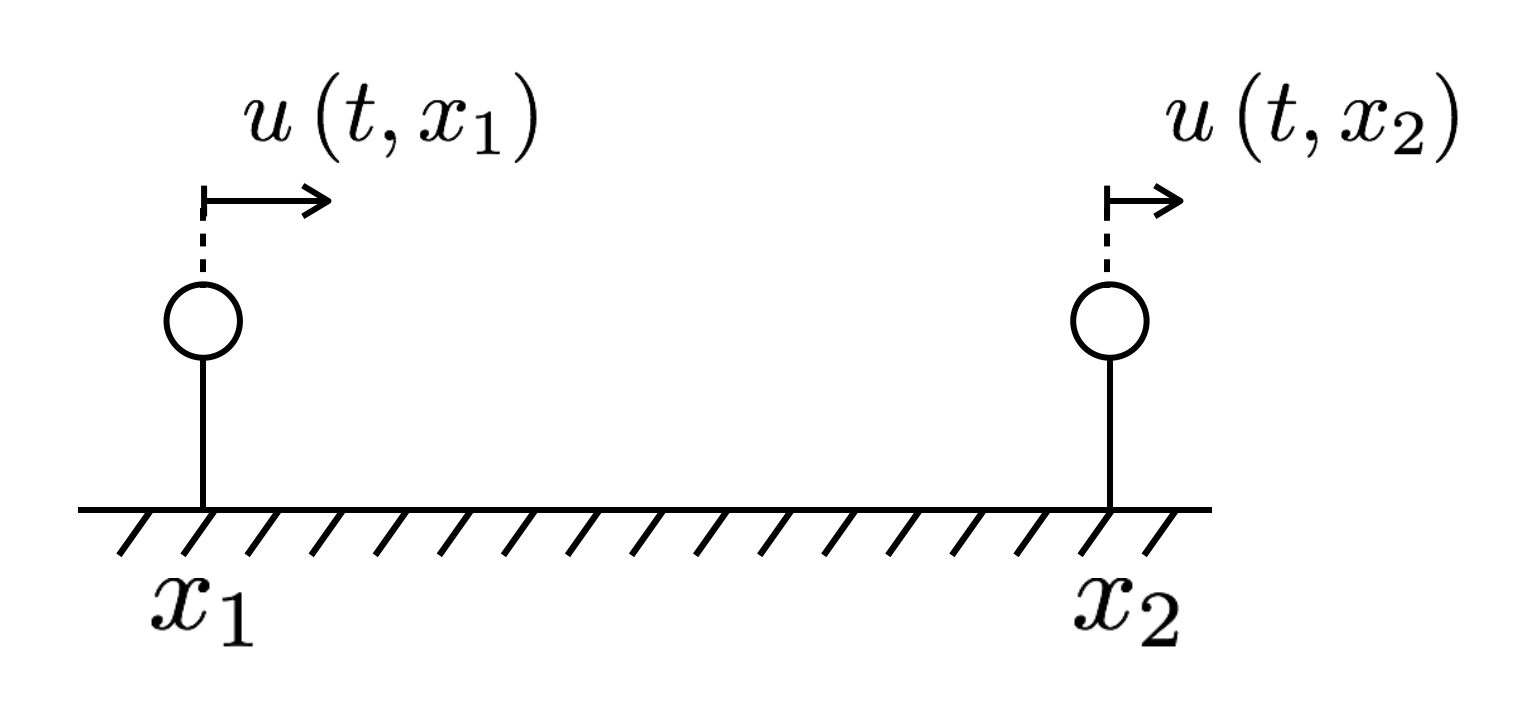
\includegraphics[width=11.0cm]{./img_cdmr_xarm.png}
  \end{center}
  \caption{\textbf{(Caution!! This plot shows the case of single plane wave.)} CDMR in the case of the uniform plane wave model.(Upper) The amplitude spectrum densities of the differential and common motion in X arm cavity which is measured by seismometers near the each ITMX and ETMX chambers. (Lower) CDMR which is a ratio of the amplitudes of the common motion over differential motion, is shown in black line. Green Line is CDMR in the case the uniform plane wave model. Blue line is CDMR with no correlation between each mirrors.}\label{img:img_cdmr_xarm}
\end{figure}

Fig.(\ref{img:img_cdmr_xarm}) shows the CDMR in the X-arm wih the uniform plane wave model. To compute the CDMR defined in Eq.(\ref{eq:eq23}), these ASDs of differential and common motion are calcutated with the timeseries signals of seismometers using Eq.(\ref{eq:eq22}) before FFT. 





\subsection{Comparizon with surface detectors}
I'm tired. I'll write tomorrow.

\subsubsection{Phase Velocity Estimation}

\begin{figure}[H] 
 \begin{minipage}{0.5\hsize}
  \begin{center}
    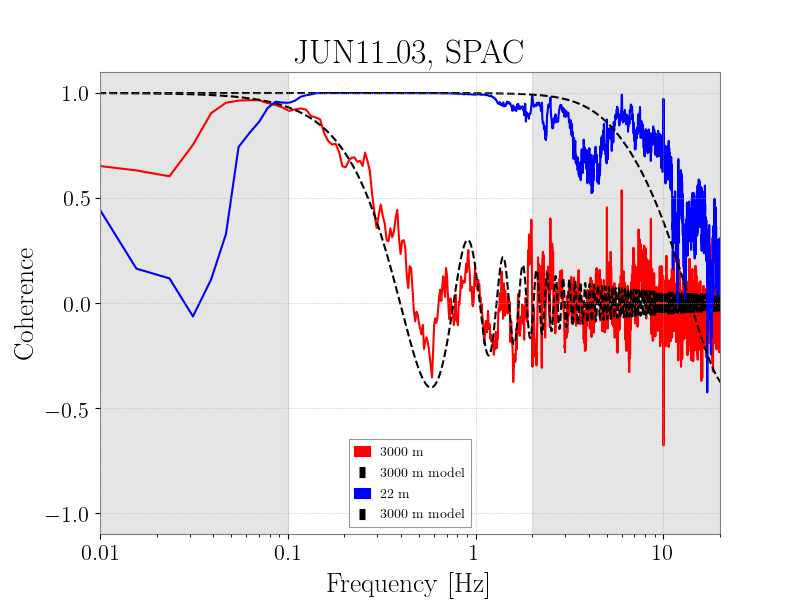
\includegraphics[width=8.0cm]{./img_coherence_result.png}    
  \end{center}
  \subcaption{}  
  \label{img:img_coherence_result}
 \end{minipage}
 \begin{minipage}{0.5\hsize}
  \begin{center}
    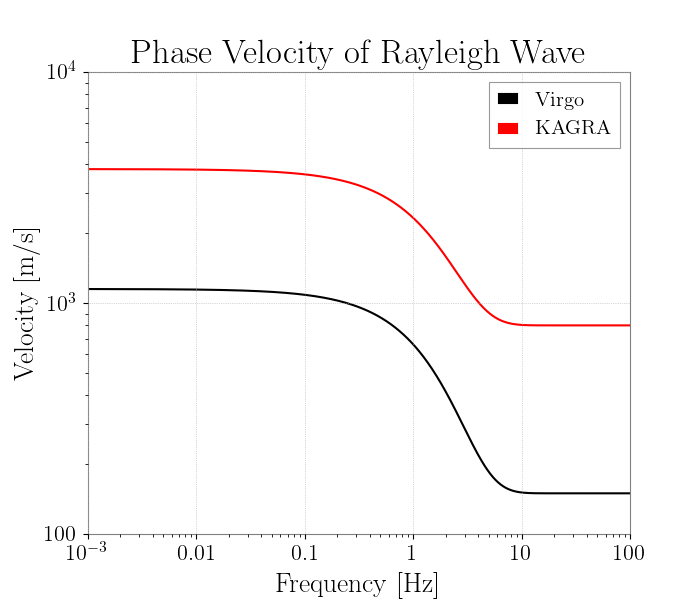
\includegraphics[width=8.0cm]{./img_RwaveVelocity.png}    
  \end{center}
  \subcaption{}
  \label{img:img_RwaveVelocity}  
 \end{minipage}
  \caption{(a) The complex coherence between two locations. Red solid line is a complex coherence in 3000 m distance. Blue one is a coherence in 22 m distance. Black dashed line is given by Eq.(\ref{eq:eq19}) with asuming a profile of the phase velocity on Fig.(\ref{img:img_RwaveVelocity}). (b) The phase velocity of the Rayleigh wave. Black solid line is sited from M.Beker's PhD thesis. Red one is taken by fitting the measured data on Fig.(\ref{img:img_coherence_result})} 
\end{figure}

\subsubsection{}


\begin{figure}[H]
  \begin{center}
    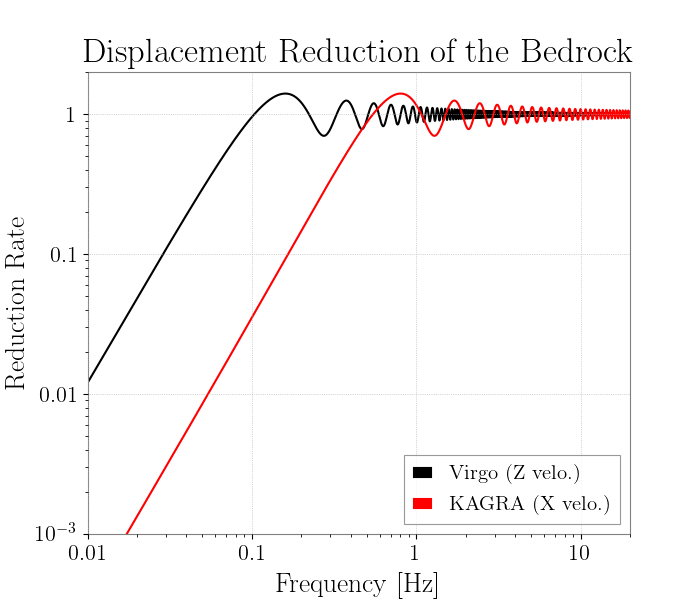
\includegraphics[width=9.5cm]{./img_CDMR.png}
  \end{center}
  \caption{Comparizon of the Reduction effect between KAGRA and Virgo. Eq.(\ref{eq:eq34}) with the phase velocity on the Fig.(\ref{img:img_RwaveVelocity})}
  \label{img:img_dmrr}
\end{figure}


\section{Summary of the Chapter}

\appendix

\bibliography{./cdmr_reference}

\end{document}
